\documentclass[10pt]{article}
\usepackage[letterpaper,margin=0.8in]{geometry}
\usepackage[T1]{fontenc}
\usepackage{lmodern}
\usepackage{microtype}
\usepackage{booktabs}
\usepackage{tabularx}
\usepackage{array}
\usepackage{amsmath,amssymb}
\usepackage{enumitem}
\usepackage{fancyvrb}
\usepackage{float}
\usepackage{url}
\usepackage[hidelinks]{hyperref}
\usepackage{titlesec}
\usepackage{caption}
\usepackage{xcolor}
\usepackage{tikz}
\usepackage{pgfplots}
\pgfplotsset{compat=1.18}
\usetikzlibrary{positioning,arrows.meta,fit}
\setlength{\parindent}{1.2em}
\setlength{\parskip}{0pt}
\setlist{nosep,leftmargin=1.6em}
\captionsetup{font=small}
\titleformat{\section}{\large\bfseries}{\thesection}{0.6em}{}
\titleformat{\subsection}{\normalsize\bfseries}{\thesubsection}{0.6em}{}
\newcolumntype{Y}{>{\raggedright\arraybackslash}X}
\newcommand{\SCG}{Security Coverage Graph (SCG)}
\newcommand{\code}[1]{\texttt{#1}}

\title{\textbf{The Security Coverage Graph:}\\[2pt]\large Instance-Grounded, Operability-Aware Modeling of Defensive Posture}
\author{Haodong Ji\\\texttt{edwardwang@detecteng.ai}}
\date{}

\begin{document}
\maketitle

\begin{abstract}
Defensive coverage is commonly reported at the MITRE ATT\&CK technique level, where a technique may appear covered if a detection is mapped to it. This can overstate security posture in two ways. First, coverage varies across assets: a technique covered on one system may be a gap on another. Second, a mapped detection is only useful if the affected asset produces the telemetry that detection requires.

We present the Security Coverage Graph (SCG), a graph data model that represents coverage at the (asset, technique) level. The SCG connects each threat instance to the asset's actual telemetry, deployed detections, and implemented controls. This allows it to identify false coverage, distinguish preventive coverage from detection-only partial coverage, and represent unknown states when available evidence is insufficient. The model also separates recommended controls from observed implementations and supports counterfactual analysis of changes to detections and telemetry.

We demonstrate these capabilities on a worked enterprise estate and evaluate scalability to $2\times10^5$ threat instances and approximately $10^6$ edges. The results show that coverage queries remain linear in graph size because coverage is computed from local graph relationships rather than attack-path enumeration.
\end{abstract}

\section{Introduction}
Security operations teams often answer ``what can we detect?'' with ATT\&CK-based matrices. The MITRE ATT\&CK Navigator~[1] and DeTT\&CT~[2] are widely used to visualize technique-level coverage. These views are easy to read and easy to overstate. Practitioner commentary repeatedly warns against reading ``100\% coverage'' literally---a cell can be green because a rule is mapped, not because it would fire in the environment---and notes that such maps go stale ``the moment your Sysmon config changes.''

We attribute these problems to the use of the wrong unit of analysis rather than to defects in the tooling. Coverage is reported per technique; it is actually a property of two finer things the technique cell averages away:
\begin{enumerate}
\item \textbf{The asset.} A technique cell is green if any asset detects the technique. ``T1566 is covered'' can mean it is covered for the mail gateway and a blind spot for every cloud identity, yet the cell reads one color for all of them.
\item \textbf{The data path.} A detection covers an asset only if the asset emits the telemetry that detection consumes. A phishing rule keyed on mail-flow logs does not cover an identity provider that produces no mail flow, however correctly the rule is mapped to T1566.
\end{enumerate}

Consider the AWS case used in our worked estate. An S3 mass-download detection is mapped to ATT\&CK T1530 and depends on CloudTrail S3 data events. If those data events are not enabled for the AWS asset, the rule remains present and mapped but cannot observe the relevant data-plane activity. A technique-level map can therefore remain green while the asset-specific detection path is inoperable. The same structural failure appears in Google Cloud when a rule depends on Data Access logs that are disabled. The SCG records the detection mapping and its required telemetry separately so these conditions surface as false coverage.

The \SCG{} is a graph model built to make these the first-class units. Its canonical node is the ThreatInstance, a single (asset, technique, version) tuple. Detections and controls attach to instances, never to assets or techniques directly. The asset's telemetry production is itself modeled as edges (App $\rightarrow$ PRODUCES $\rightarrow$ Telemetry $\rightarrow$ POWERS $\rightarrow$ Detection), with POWERS edges grouped into conjunctive telemetry requirements. If no requirement group is fully satisfied for a mapped detection, the mapping is false coverage, computed as a graph anti-join statically and continuously rather than by running an attack.

The graph does not model detective coverage alone; for each instance it carries detective coverage, mitigative coverage (controls actually implemented), and a distinct prescriptive reference layer (what ATT\&CK recommends). Accordingly, the model represents the defensive posture of an asset against a technique, not detective coverage alone.

\paragraph{Contributions.} We make five claims, each grounded in a concrete mechanism of the model and supported by a query (Sections~3--6):

\paragraph{(T1) Instance-grounded coverage.} The correct unit is the (asset, technique) instance; technique-level maps overstate posture by aggregation. We quantify the aggregation gap, the fraction of asset-technique pairs a green technique cell conceals (\S3.2, \S5).

\paragraph{(T2) False coverage as a graph anti-join.} Detection validity requires the asset to satisfy at least one telemetry requirement group; ``paper coverage'' is an automatically detectable anti-join with no analog in technique-level mappings (\S3.3, \S5).

\paragraph{(T3) Epistemically explicit posture.} Coverage must distinguish gap (checked, absent) from unknown (could not check), with unknown tied to collector provenance rather than to test coverage. The combined posture remains four-state: covered, partial, gap, or unknown (\S3.4).

\paragraph{(T4) Prescriptive vs. observed.} The model separates what the framework recommends from what the environment implements, and the corresponding analytic computes their difference (\S3.5).

\paragraph{(T5) Simulatable, provenance-bearing posture.} Coverage is a continuously reconciled database with per-write provenance and read-only counterfactual simulation, not a hand-maintained artifact (\S3.6).

Graph population is outside the scope of this paper. Mechanical connectors, analyst edits, and an LLM agent can all write through the same interface; the contributions here depend on the graph invariants and coverage analytics. Agentic population is deferred to companion work.

\section{Related Work}
We group prior art into five traditions and state, for each, what it provides and where it stops.

\paragraph{Technique-level coverage annotation.} The ATT\&CK Navigator~[1] provides matrix-layer annotation. DeTT\&CT~[2] adds separate scoring of data-source quality, visibility, and detection, and can scope multiple scores for a technique to different system types using \code{applicable\_to}. These remain technique-centered coverage annotations; they do not bind an environment-specific asset-technique instance to the asset's live telemetry-to-detection path and implemented controls.

\paragraph{Sensors, data sources, and detection robustness.} MITRE's Center for Threat-Informed Defense is closest on the data side. Sensor Mappings to ATT\&CK~[3] maps concrete sensor events to ATT\&CK data sources/components; Summiting the Pyramid~[4] quantifies detection robustness and telemetry confidence; ATT\&CK's Data Sources / Data Components and OSSEM~[5] formalize the technique$\rightarrow$data-component relationships our overlay imports. These identify which telemetry could detect a technique in general; they do not model whether a specific asset actually emits that telemetry into the specific detection. The mapping is technique$\rightarrow$data-source (catalog-level), not asset$\rightarrow$telemetry$\rightarrow$detection (instance-grounded).

\paragraph{Empirical validation (BAS / adversary emulation).} Breach-and-attack simulation and Atomic Red Team~[6] validate coverage by executing technique procedures and observing whether detections fire, catching the ``rule exists but does not fire'' case directly. BAS is episodic and intrusive: it identifies failures observed during testing, not a continuously maintained, queryable model of why coverage is present.

\paragraph{Detection-engineering theory.} SpecterOps's Capability Abstraction~[7] and Funnel of Fidelity~[8], and the detection-as-code movement, give the vocabulary for building a good detection. This tradition is about how to build one detection well; it is largely silent on modeling the coverage of a whole estate as data.

\paragraph{Security knowledge graphs.} A mature academic literature models cybersecurity knowledge as graphs: D3FEND~[9] (countermeasures), AttacKG~[10] (technique graphs from CTI reports), ATT\&CK-to-CVE pipelines, and surveys~[11]; a SoK on ATT\&CK in research and practice~[12] identifies gaps in practical implementation and evaluation. Classical attack graphs (e.g., MulVAL~[13]) model reachability of attacker states. These model threat knowledge (mostly normative/global) or attacker reachability; they are not defensive-posture graphs of a specific environment that bind a live asset inventory, its actual telemetry production, its deployed detections, and its implemented controls into one instance-grounded model of operable coverage.

\paragraph{The gap.} Across all five traditions (Table~\ref{tab:related}), no prior system makes the unit of coverage the (asset, technique) instance, binds it to the asset's actual telemetry and actually implemented controls, and computes operability continuously from live inventory with provenance.

\begin{table}[t]
\centering
\small
\begin{tabularx}{\linewidth}{@{}Y l c c c@{}}
\toprule
Tradition & Unit of analysis & Env-specific? & Operability? & Maintained?\\
\midrule
Navigator / DeTT\&CT & technique / system-scoped score & partial & no & manual / automatable\\
SMAP / STP / OSSEM & tech. $\rightarrow$ data src & no (catalog) & partial & no (ref.)\\
BAS / Atomic & tech. procedure & when tested & episodic & test-time\\
SpecterOps / ADS & one detection & n/a & per-det. & n/a\\
Academic KGs & threat knowledge & mostly global & no & varies\\
SCG (ours) & (asset, tech.) & yes & yes (graph) & continuous\\
\bottomrule
\end{tabularx}
\caption{Where prior traditions stop, and the SCG's niche.}
\label{tab:related}
\end{table}

\begin{table}[t]
\centering
\small
\begin{tabularx}{\linewidth}{@{}l l Y@{}}
\toprule
Edge & From $\rightarrow$ To & Meaning\\
\midrule
HAS\_TI & App $\rightarrow$ ThreatInstance & asset is at risk of technique\\
DESCRIBES & TTP $\rightarrow$ ThreatInstance & technique of the instance\\
DETECTED\_BY & ThreatInstance $\rightarrow$ Detection & a detection is mapped\\
PRODUCES & App $\rightarrow$ Telemetry & asset emits this telemetry\\
POWERS & Telemetry $\rightarrow$ Detection & telemetry is a member of a requirement group\\
HAS\_CI & App $\rightarrow$ Ctrl.Inst. & control deployed on asset\\
IMPLEMENTED\_BY & Control $\rightarrow$ Ctrl.Inst. & catalog control realized\\
MITIGATED\_BY & ThreatInstance $\rightarrow$ Ctrl.Inst. & mitigates this instance\\
MITIGATED\_BY\_REF & TTP $\rightarrow$ Mitigation & ATT\&CK recommends\\
DETECTED\_VIA & TTP $\rightarrow$ Data Comp. & ATT\&CK data ref.\\
\bottomrule
\end{tabularx}
\caption{Coverage-bearing edges. Detective coverage requires both a DETECTED\_BY edge and a satisfied telemetry requirement group; POWERS edges carry a \code{requirement\_group} property. All telemetry in one group is required, while separate groups are alternative ways to power a detection.}
\label{tab:edges}
\end{table}

\section{The Security Coverage Graph}
\subsection{Entities and edges}
The SCG is a property graph over a small, fixed schema. The nodes are: App (an environment asset such as a cloud instance, identity, bucket, or role), TTP (an ATT\&CK technique), the canonical ThreatInstance, Detection, Control and its environment-bound ControlInstance, and Telemetry (a log/data source the environment produces). A small ATT\&CK overlay (tactic, mitigation, \code{data\_source}, \code{data\_component}) is imported with provenance as a normative reference. The edges that carry the coverage semantics are summarized in Table~\ref{tab:edges} and the full schema, including both coverage arms, is drawn in Figure~\ref{fig:schema}.

\subsection{Instance-grounded coverage (T1)}
The ThreatInstance (identified canonically by \code{app\_id:ttp\_id:version\_id}) is the unit of coverage. ThreatInstances are instantiated for TTPs considered applicable to an asset's practical use in its environment. Applicability is context-dependent and supplied to SCG by security engineers, threat modeling, automated tooling, or other graph writers; SCG evaluates posture over that supplied set rather than claiming completeness over the full ATT\&CK technique universe. Each instance stores both a computed status and an effective status in \{covered, partial, gap, unknown\}; status rolls up from instances, never down to them. The default computed status follows a defensive precedence:

\begin{Verbatim}[fontsize=\small]
preventive control                                  -> covered
else operable detection                             -> partial
else detection could use only unconfirmed telemetry -> unknown
else                                                 -> gap
\end{Verbatim}

A preventive control therefore makes an instance covered by default even when no detection is present: the modeled attack path is considered prevented. In the current implementation, ControlInstance has no separate sync state, so the presence of a preventive ControlInstance is treated as confirmed. Detection alone is partial because the technique may still succeed even though its execution should be observable. An optional security-engineer override may replace the computed status when structural control presence overstates real effectiveness or scope. Every override must carry an engineer's identity, reason, and timestamp so the effective status remains auditable. The effective status is the override when one exists; otherwise it is the computed status.

\begin{figure}[t]
\centering
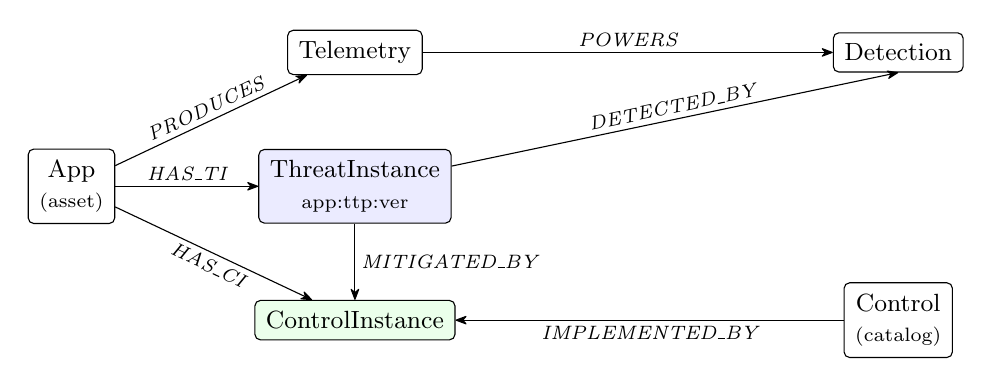
\begin{tikzpicture}[
  >={Stealth[round]},
  every node/.style={font=\small},
  box/.style={draw, rounded corners=2pt, inner sep=4pt, align=center},
  inst/.style={box, fill=blue!8},
  cinst/.style={box, fill=green!8},
  rel/.style={font=\scriptsize\itshape, inner sep=2pt}]
  % spine
  \node[box]  (app) at (0,0)     {App\\\scriptsize(asset)};
  \node[inst] (ti)  at (3.6,0)   {ThreatInstance\\\scriptsize app:ttp:ver};
  % detection arm (upper)
  \node[box]  (tel) at (3.6,1.7) {Telemetry};
  \node[box]  (det) at (10.5,1.7) {Detection};
  % control arm (lower)
  \node[cinst] (ci)   at (3.6,-1.7) {ControlInstance};
  \node[box]   (ctrl) at (10.5,-1.7) {Control\\\scriptsize(catalog)};
  % spine edge
  \draw[->] (app) -- node[rel,above]{HAS\_TI} (ti);
  % detection arm
  \draw[->] (app) -- node[rel,above,sloped]{PRODUCES} (tel);
  \draw[->] (ti)  -- node[rel,above,sloped,pos=0.5]{DETECTED\_BY} (det.south);
  \draw[->] (tel) -- node[rel,above]{POWERS} (det.west);
  % control arm
  \draw[->] (app)  -- node[rel,below,sloped]{HAS\_CI} (ci);
  \draw[->] (ti)   -- node[rel,right]{MITIGATED\_BY} (ci);
  \draw[->] (ctrl) -- node[rel,below]{IMPLEMENTED\_BY} (ci);
\end{tikzpicture}
\caption{Instance-grounded coverage schema. Both defensive arms attach to the ThreatInstance rather than to App or TTP directly.}
\label{fig:schema}
\end{figure}

Both defensive arms attach to the ThreatInstance rather than to App or TTP directly. A DETECTED\_BY edge is operable only when the same app supplies every telemetry input in at least one POWERS requirement group and those telemetry inputs are confirmed; otherwise its requirement state is either absent or unknown (\S3.3). A preventive ControlInstance makes the computed status covered by default. If no preventive control is present, an operable detection yields partial; if no detection is operable but at least one mapped detection could be powered only by currently unconfirmed telemetry, the instance is unknown; otherwise it is a gap. A security-engineer override may replace the computed state when the deployed control does not fully prevent the relevant technique.

\paragraph{What is an ``asset''?} The App node is modeled at the coarsest granularity whose members share the same telemetry production, controls, and hence coverage---a coverage-equivalence class. This lands at different levels for different asset kinds: a named platform carries vendor identity (an Entra tenant and an Okta tenant emit different logs and are distinct Apps), while a fleet of endpoints need not be enumerated per host or collapsed into a single node because instrumentation varies. Instead, it can be split into categories, such as a managed EDR-and-Sysmon workstation class and a legacy class with only the Windows Security log. Aggregating assets into a class is exactly the move T1 warns against at the technique level, but it is lossless precisely when the class is coverage-homogeneous: the class is the level at which within-cell coverage variance is zero. The instance grounding is therefore not an arbitrary granularity choice; it is the coarsest aggregation that conceals no gap. The aggregation gap below measures what the next coarser step, the technique, destroys.

A technique-level view is then a derived, lossy aggregation. Because the heatmap being compared is a detective-coverage view, its aggregation gap is defined over detective operability rather than the four-state combined posture. The metric counts instances with absent detective coverage whose technique-level cell is still green, divided by all instances. Unknown instances are reported separately rather than coerced into gaps:
\begin{Verbatim}[fontsize=\small]
function aggregation_gap(instances):
    hidden_gaps = 0
    for i in instances:
        if detective_state(i) == ABSENT
           and technique_cell(ttp(i)) == GREEN:
            hidden_gaps += 1
    return hidden_gaps / count(instances)
\end{Verbatim}
This is the quantity a green technique heatmap conceals, and it is computable only because coverage lives at the instance.

\subsection{False coverage as a graph anti-join (T2)}
A mapped detection may require multiple telemetry inputs. Each POWERS edge carries a \code{requirement\_group} property: telemetry in the same group is conjunctive (AND), while separate groups are alternatives (OR). An omitted group identifier defaults to group 1. Requirement state and false coverage are computed as follows:
\begin{Verbatim}[fontsize=\small]
function requirement_state(app, detection):
    saw_unknown = false
    for group in requirement_groups(detection):
        if all(app PRODUCES t and t.sync_state == CONFIRMED
               for t in group):
            return OPERABLE
        if all(app PRODUCES t for t in group)
           and any(t.sync_state == UNCONFIRMED for t in group):
            saw_unknown = true
    if saw_unknown:
        return UNKNOWN
    return ABSENT

function false_coverage(instance, detection):
    return DETECTED_BY(instance, detection)
           and requirement_state(app(instance), detection) == ABSENT
\end{Verbatim}
Thus a rule requiring both process and network telemetry is not operable when only one is present; alternative telemetry implementations are represented as separate requirement groups. A mapped detection whose only potentially satisfiable requirement group depends on unconfirmed telemetry is unknown rather than false coverage.


\begin{figure}[H]
\centering
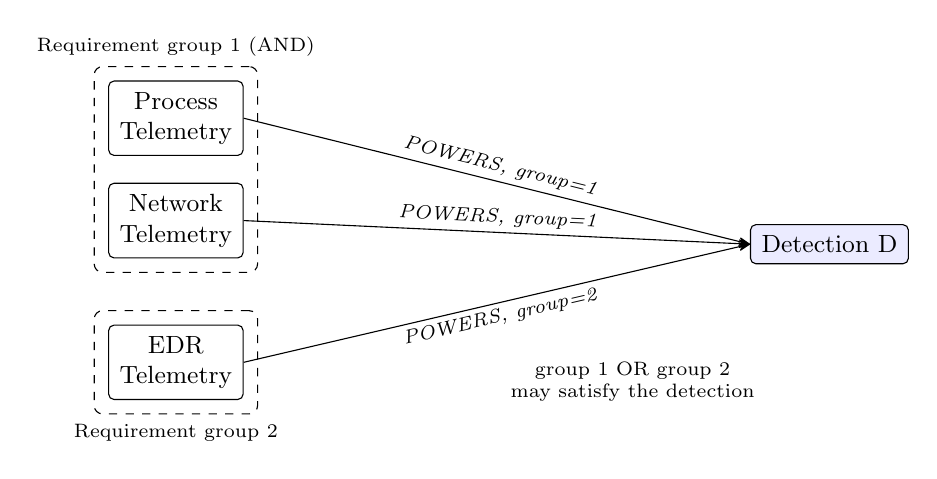
\begin{tikzpicture}[
  >={Stealth[round]},
  every node/.style={font=\small},
  box/.style={draw, rounded corners=2pt, inner sep=4pt, align=center},
  group/.style={draw, dashed, rounded corners=3pt, inner sep=5pt},
  rel/.style={font=\scriptsize\itshape, inner sep=2pt}]
  \node[box] (proc) at (0,1.1) {Process\\Telemetry};
  \node[box] (net)  at (0,-0.2) {Network\\Telemetry};
  \node[box] (edr)  at (0,-2.0) {EDR\\Telemetry};
  \node[box, fill=blue!8] (det) at (8.3,-0.5) {Detection D};

  \node[group, fit=(proc)(net), label={[font=\scriptsize]above:Requirement group 1 (AND)}] (g1) {};
  \node[group, fit=(edr), label={[font=\scriptsize]below:Requirement group 2}] (g2) {};

  \draw[->] (proc.east) -- node[rel,above,sloped]{POWERS, group=1} (det.west);
  \draw[->] (net.east)  -- node[rel,above,sloped]{POWERS, group=1} (det.west);
  \draw[->] (edr.east)  -- node[rel,below,sloped]{POWERS, group=2} (det.west);

  \node[font=\scriptsize, align=center] at (5.8,-2.25) {group 1 OR group 2\\may satisfy the detection};
\end{tikzpicture}
\caption{Telemetry requirement groups for one detection. Inputs in the same POWERS group are conjunctive; separate groups are alternatives. Here the detection is operable with both process and network telemetry, or with EDR telemetry alone.}
\label{fig:reqgroups}
\end{figure}

This condition is evaluated as an anti-join over the graph; no rule is executed and no attack is launched. The \code{telemetry\_sources} string field on a detection is informational, while POWERS plus the app's PRODUCES relationships and telemetry sync state are authoritative for operability. Discounting false-coverage edges can demote a detection-only instance from partial to gap when its last operable detection disappears; if another operable detection remains, the instance stays partial. A mapped detection that depends only on unconfirmed telemetry instead contributes an unknown state and is excluded from false-coverage results. A preventive control keeps the default computed status covered, subject to an explicit security-engineer override. The recompute is edge-local.

\subsection{Epistemically explicit posture (T3)}
Conflating ``we checked and there is no telemetry'' with ``we could not check'' miscalibrates posture. The SCG represents epistemic state as a first-class value: \code{telemetry.sync\_state} $\in$ \{confirmed, unconfirmed\} with an \code{unconfirmed\_reason}. When a telemetry source becomes unconfirmed, its structural PRODUCES and POWERS relationships are retained for provenance, but paths involving that telemetry no longer count as evidence of operability or absence. When no preventive control exists, an instance whose candidate detection could be powered only through such unconfirmed telemetry is unknown rather than gap: the model lacks enough evidence to say the detective path is absent. When a preventive control is present, the default computed status remains covered; a security engineer may still override that status when the control is known not to prevent the relevant procedure or scope. Thus unknown is an epistemic state, not a third replacement for covered/partial/gap, and it remains tied to collector provenance (the \code{sync\_session} audit of whether a connector run was ok / error / stale\_source) rather than to test coverage.

\subsection{Prescriptive vs. observed (T4)}
The model separates MITIGATED\_BY\_REF (TTP $\rightarrow$ MITRE Mitigation, what is recommended) from MITIGATED\_BY (instance $\rightarrow$ concrete ControlInstance, what is implemented). The corresponding recommendation-gap query returns each (app, ttp, recommended-mitigation) triple with no implemented control. A current limitation is that the reference$\leftrightarrow$implementation match uses a case-insensitive substring comparison between mitigation and control names. More reliable normative-to-observed mapping remains open work.

\subsection{Simulatable, provenance-bearing posture (T5)}
Static annotation (YAML/JSON heatmaps) can become stale and is difficult to audit. The SCG addresses this by being (a) synced from live inventory: structured connectors pull cloud assets from cartography (App/Telemetry/PRODUCES) and detections from the SIEM; (b) provenance-stamped: every synced row carries \code{last\_synced\_at} / \code{synced\_by} and every run is audited in \code{sync\_session}; and (c) simulatable: \code{impact\_analysis()} is a read-only deletion simulation that asks, ``if I retire this detection or decommission this telemetry source, which instances degrade?'' It is computed over an in-memory edge index without mutating the database. These checks apply to any graph writer and therefore belong to the data model rather than to a particular population mechanism.

\section{Coverage Query Semantics}
The contributions reduce to a handful of queries with the complexities in Table~\ref{tab:complexity}. None of them require path enumeration or transitive closure: every coverage question is answered by local incidence (does this instance have the right edges?) or by a single anti-join. Per-instance status is materialized on write, so reading posture at rest is $O(1)$ per instance; a coverage-edge write recomputes only the ThreatInstances affected by that edge.

\begin{table}[t]
\centering
\small
\begin{tabularx}{\linewidth}{@{}Y l Y@{}}
\toprule
Query & Complexity & Scales with\\
\midrule
per-instance status & $O(1)$ (materialized) & read at rest\\
\code{impact\_analysis(n)} & $O(\mathrm{nbhd}(n))$ & local fan-out\\
edge write $\rightarrow$ recompute & $O(k)$ & affected local fan-out\\
\code{false\_coverage(app)} & $O(\text{instances of app})$ & one app\\
\code{false\_coverage()} & $O(|\text{detections}|)$ & number of detections\\
\code{list\_*\_gaps()} & $O(|\text{instances}|)$ & number of instances\\
\bottomrule
\end{tabularx}
\caption{Query complexity. Coverage is local; the costliest analytic (false coverage) scales with the smaller dimension (deployed detections), not the asset count.}
\label{tab:complexity}
\end{table}

\section{Worked Enterprise Scenarios}
We exercise the model on a canonical seed estate representing a hybrid enterprise of 8 apps: two endpoint categories (managed and legacy), on-prem Active Directory, Entra, AWS, GCP, a web application, and a web-application firewall. The estate spans 8 ATT\&CK (sub)techniques and 13 relevant (asset, technique) instances. Metrics are produced by \code{metrics/scg\_metrics.py}.

The estate is hand-authored and the percentages below are illustrative rather than population estimates. Apps are modeled as coverage-equivalence classes, and the scenarios use common configuration failures represented directly in the seed: legacy hosts without EDR/Sysmon, CloudTrail S3 data events left disabled, and GCP Data Access logs off by default. The identical harness runs on a real cartography-fed \code{dcg.db}; producing population-level figures remains future work (\S7).

\paragraph{Scenario 1---cloud storage exfiltration with missing audit logs.} Consider detections for mass object downloads in AWS and Google Cloud. The AWS T1530 detection expects CloudTrail S3 data events, while the GCP T1530 detection expects GCP Data Access logs. In the seed, those telemetry sources are not enabled for the corresponding assets. The detections remain mapped to the technique, but neither asset can satisfy the required telemetry path. This is the T2 false-coverage condition: \code{false\_coverage\_check()} returns three data-starved mappings overall (Table~\ref{tab:false}), representing 25\% of all DETECTED\_BY edges (3/12) and affecting 27.3\% of detection-bearing instances. AWS $\cdot$ T1530 would otherwise compute as covered because S3 Block Public Access is present, but the seed carries an explicit engineer override to partial because that control does not prevent an authenticated principal from performing the relevant mass-download procedure; GCP $\cdot$ T1530 falls to gap once the inoperable detection is discounted. The same structural failure therefore appears across two cloud platforms even though the concrete log sources differ.

\begin{table}[t]
\centering
\small
\begin{tabularx}{\linewidth}{@{}l l Y@{}}
\toprule
Instance & Detection & Powered by telemetry the app lacks\\
\midrule
AWS $\cdot$ T1530 & S3 Mass Download & CloudTrail S3 data events (not enabled)\\
EP-Cat-B $\cdot$ T1003.001 & LSASS (Sysmon) & Sysmon (legacy host runs none)\\
GCP $\cdot$ T1530 & GCS Bulk Egress & GCP Data Access logs (off by default)\\
\bottomrule
\end{tabularx}
\caption{False coverage on the seed: mapped detections that cannot fire for the asset because the at-risk app does not produce the powering telemetry, found by a graph anti-join with no execution.}
\label{tab:false}
\end{table}

The same cloud estate also exercises the prescriptive-versus-observed distinction in T4. The recommendation-gap query returns 17 (app, technique, missing-mitigation) triples by diffing MITRE's recommended mitigations against implemented controls. For cloud-account abuse, AWS implements privileged-access management but lacks the MFA mitigation represented in Entra; Entra implements MFA but lacks the privileged-access-management mitigation represented in AWS. This remains subject to the current substring-matching limitation in \S3.5, and fronting controls such as the web application's WAF are not credited across assets (\S7).

\paragraph{Scenario 2---technique-level coverage hides heterogeneous assets.} The seed also shows how a green technique cell can hide materially different posture across asset classes. A technique-level view reports the estate as 100\% detected (8/8 techniques) and 75\% fully covered (6/8). The operability-aware instance view reports 61.5\% detection coverage (8/13) and 46.2\% full coverage (6/13), with effective status distribution 6 covered / 3 partial / 4 gap. Thus 38.5\% of asset-technique pairs lack operable detective coverage beneath a green technique cell, and 37.5\% of techniques are heterogeneous in effective posture. T1566.002 is covered on the managed endpoint class but a gap on the legacy class; T1078.004 is covered on Entra and AWS but a gap on GCP. T1530 is also heterogeneous: AWS is partial by engineer override while GCP is a gap. Figure~\ref{fig:aggregation} shows two representative examples.

\begin{figure}[H]
\centering
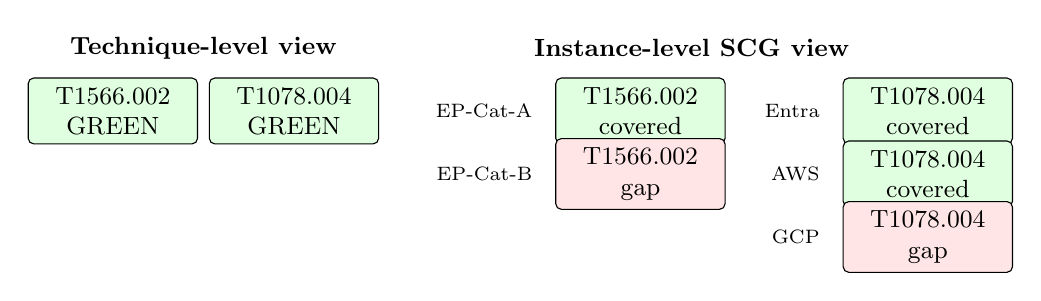
\begin{tikzpicture}[
  every node/.style={font=\small},
  box/.style={draw, rounded corners=2pt, minimum width=2.15cm, minimum height=0.62cm, align=center},
  covered/.style={box, fill=green!12},
  gap/.style={box, fill=red!10},
  label/.style={font=\scriptsize}]
  \node[font=\small\bfseries] at (-3.2,2.25) {Technique-level view};
  \node[covered] at (-4.35,1.45) {T1566.002\\GREEN};
  \node[covered] at (-2.05,1.45) {T1078.004\\GREEN};

  \node[font=\small\bfseries] at (3.0,2.25) {Instance-level SCG view};
  \node[label, anchor=east] at (1.10,1.45) {EP-Cat-A};
  \node[covered] at (2.35,1.45) {T1566.002\\covered};
  \node[label, anchor=east] at (1.10,0.65) {EP-Cat-B};
  \node[gap] at (2.35,0.65) {T1566.002\\gap};

  \node[label, anchor=east] at (4.75,1.45) {Entra};
  \node[covered] at (6.00,1.45) {T1078.004\\covered};
  \node[label, anchor=east] at (4.75,0.65) {AWS};
  \node[covered] at (6.00,0.65) {T1078.004\\covered};
  \node[label, anchor=east] at (4.75,-0.15) {GCP};
  \node[gap] at (6.00,-0.15) {T1078.004\\gap};
\end{tikzpicture}
\caption{Technique-level aggregation can remain green while individual asset-technique instances contain gaps. The figure shows two representative heterogeneous techniques from the worked estate.}
\label{fig:aggregation}
\end{figure}

The endpoint example also exposes the T3 distinction between gap and unknown. When each collector is treated as failed in turn, 7 of 8 operably detected instances are single-source fragile at the detective layer: a collector failure makes their detective evidence unknown rather than proving a gap. The managed endpoint class is the exception for LSASS credential access (T1003.001), where both EDR and Sysmon back the detection path. The legacy endpoint has no such redundancy.

\paragraph{Scenario 3---change impact before decommissioning telemetry.} T5 also turns telemetry retirement into an operational change-management question: what happens if \code{tel:ds-repl} is decommissioned? The \code{impact\_analysis()} query uses the same operability-aware status logic and reports one degraded ThreatInstance: AD $\cdot$ T1003.006 moves from partial to gap because its detection path loses the telemetry that made it operable. The graph answers this question read-only, before the telemetry source is removed from the environment.

\section{Scaling}
At larger graph sizes ($\sim$300k nodes), scalability depends on both the model and its implementation.

\subsection{Why the model is linear}
The node budget is dominated by App (cloud assets: $10^4$--$10^5+$) and ThreatInstance ($O(\text{relevant app}\times\text{technique pairs})$). ThreatInstances are the main multiplier in a 300k-node graph but remain sparse because they exist only for relevant pairs. Everything else (techniques + overlay $\approx$1k, telemetry $\approx$dozens, detections $\approx$hundreds) is bounded.

Classical attack graphs encode coverage over attack paths, where multi-hop reachability can produce a worst-case exponential number of paths in hosts and vulnerabilities. The SCG models a different question. Coverage of an instance is local: does it have a mapped detection with a satisfied telemetry requirement group, or an applicable MITIGATED\_BY edge under the status precedence? No path enumeration, no transitive closure, no fixpoint. Every query is linear or sub-linear in the data it touches (Table~\ref{tab:complexity}), and the costliest analytic scales with the smaller dimension. This formulation keeps coverage evaluation local and avoids path traversal. The SCG therefore addresses a different problem from classical attack graphs: coverage rather than attack-path reachability.

\subsection{Closing the implementation gap}
Benchmarking against the model exposed four places where the code did not realize its linearity: (1) \code{list\_edges()} used a \code{(? IS NULL OR col = ?)} filter idiom that forced a full scan of the edge table instead of an index seek; (2) \code{impact\_analysis()} loaded the entire edge table on every call; (3) \code{delete\_node()} ran a full \code{recompute\_coverage()} over every instance after any deletion, and its cascade scanned an unindexed column; and (4) \code{false\_coverage\_check()} was $O(n^2)$---the unique autoindex \code{(edge\_type, from\_id, to\_id)} could not seek \code{to\_id} on the Telemetry--POWERS--Detection join, degrading to a per-row scan over all POWERS edges. We fixed these by building WHERE clauses from only supplied predicates, scoping \code{impact\_analysis} to a node's neighborhood, recomputing only instances that lost a coverage edge, and adding composite indices \code{(from\_id, edge\_type)} / \code{(to\_id, edge\_type)} with an ANALYZE step so the planner chooses them. The last fix alone turned 17.1~s at $10^4$ instances into about 14~ms.

\begin{table}[t]
\centering
\small
\begin{tabular}{@{}r r r r r r@{}}
\toprule
& \multicolumn{3}{c}{neighborhood-bound (ms)} & \multicolumn{2}{c}{full-estate (ms)}\\
\cmidrule(lr){2-4}\cmidrule(l){5-6}
TIs & impact & delete & fc(app) & fc(all) & gaps\\
\midrule
1,031 & 0.059 & 0.098 & 0.041 & 1.2 & 0.1\\
10,031 & 0.057 & 0.099 & 0.042 & 14.4 & 0.8\\
50,031 & 0.058 & 0.098 & 0.042 & 75.1 & 4.5\\
100,031 & 0.059 & 0.102 & 0.041 & 153.1 & 9.3\\
200,031 & 0.058 & 0.103 & 0.044 & 330.2 & 19.8\\
\bottomrule
\end{tabular}
\caption{Scaling (medians). Neighborhood-bound operations (\code{impact\_analysis}, isolated delete, app-scoped false coverage) are flat from 1k to 200k instances; full-estate reports (whole-estate false coverage, gap listing) are linear.}
\label{tab:scaling}
\end{table}

\begin{figure}[H]
\centering
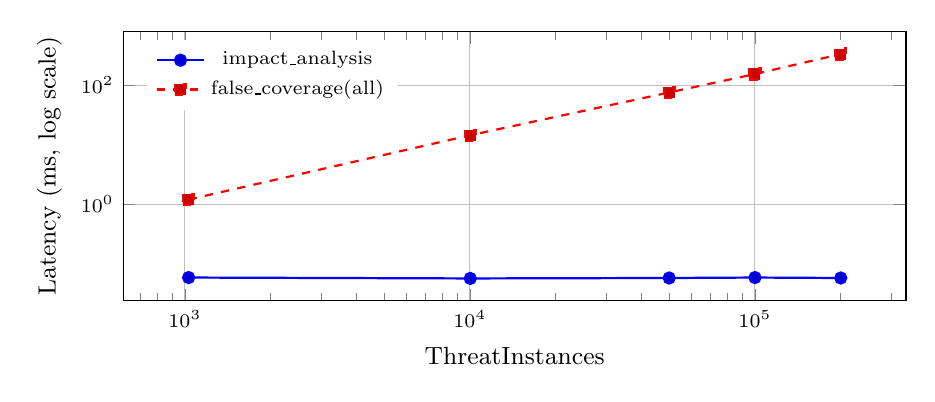
\begin{tikzpicture}
\begin{axis}[
  width=0.95\linewidth,
  height=5.0cm,
  xlabel={ThreatInstances},
  ylabel={Latency (ms, log scale)},
  xmode=log,
  ymode=log,
  log basis x=10,
  log basis y=10,
  grid=major,
  legend style={font=\scriptsize, draw=none, at={(0.03,0.97)}, anchor=north west},
  tick label style={font=\scriptsize},
  label style={font=\small}]
  \addplot+[mark=*, thick] coordinates {
    (1031,0.059) (10031,0.057) (50031,0.058) (100031,0.059) (200031,0.058)
  };
  \addlegendentry{impact\_analysis}
  \addplot+[mark=square*, thick, dashed] coordinates {
    (1031,1.2) (10031,14.4) (50031,75.1) (100031,153.1) (200031,330.2)
  };
  \addlegendentry{false\_coverage(all)}
\end{axis}
\end{tikzpicture}
\caption{Representative scaling behavior from Table~\ref{tab:scaling}. Neighborhood-bound impact analysis stays nearly flat as the graph grows, while the whole-estate false-coverage query grows approximately linearly. Both axes are logarithmic.}
\label{fig:scaling}
\end{figure}

\subsection{Measured scaling behavior}
Table~\ref{tab:scaling} reports medians produced by \code{metrics/scaling\_bench.py} on synthetic graphs from $10^3$ to $2\times10^5$ instances ($\sim10^6$ edges), using in-memory SQLite. Absolute milliseconds are machine-specific; the shape across $N$ is the result. Neighborhood-bound operations are essentially constant over a 200$\times$ size range, while full-estate reports grow approximately linearly. At 200k instances, the whole-estate false-coverage query completes in approximately 330~ms, while all neighborhood-bound operations in Table~\ref{tab:scaling} remain below 0.11~ms.

Two regression tests assert \code{impact\_analysis} and \code{delete\_node} stay sublinear as unrelated graph bulk grows, so a return to a full scan fails CI.

\section{Limitations and Threats to Validity}
\paragraph{Seed vs. real data.} The figures in \S5 are a worked demonstration on a hand-authored estate (8 apps, 13 instances), not population estimates. The identical harness runs on a real cartography-fed \code{dcg.db}; population-level prevalence is the remaining empirical step.

\paragraph{Future improvements---asset-equivalence weighting.} The current demonstration counts each App coverage-equivalence class equally, so percentages do not reflect the number or criticality of underlying assets represented by each class. Future work will report weighted coverage alongside unweighted coverage using class cardinality and, where appropriate, asset criticality or exposure.

\paragraph{Enterprise validation.} Future work will deploy the SCG in a real enterprise environment and validate sampled ThreatInstances through security-engineer review and authorized Breach and Attack Simulation (BAS), exercising the full path to observe whether a procedure is prevented, detected, or neither and comparing those outcomes with the graph-predicted status.

\paragraph{Inventory completeness.} False coverage (T2) and fragility (T3) assume the confirmed PRODUCES inventory is complete. An incomplete or unconfirmed inventory must surface as T3 unknown, not as spurious T2 false coverage. The two metrics are designed to be read together and the harness keeps them separate so the distinction stays visible.

\paragraph{Control confirmation.} The current implementation does not maintain a separate sync state on ControlInstance; presence of a preventive ControlInstance is therefore treated as confirmed. A future version should track control confirmation and collector provenance separately, analogous to telemetry, so stale or failed control inventory can surface as unknown rather than covered.

\paragraph{Fronting-infrastructure telemetry.} The PRODUCES model assumes an asset emits its own telemetry. Observability supplied by fronting infrastructure---a WAF, proxy, CASB, or API gateway that produces telemetry about another app---is not captured: the source is attributed to the fronting device, so a detection powered by it would be mis-flagged as false coverage for the observed app. Modeling this cleanly (e.g., an OBSERVES relationship the anti-join respects) is future work; the seed keeps fronting telemetry (WAF logs) off the detection path so the reported figures are undistorted.

\paragraph{Name matching (T4).} The prescriptive$\leftrightarrow$observed match is a crude case-insensitive substring match and can produce false positives. More reliable normative-to-observed mapping remains open work.

\paragraph{Operational scaling limits.} These limitations arise from the current implementation. SQLite is single-writer (WAL gives concurrent readers); a high-throughput continuous sync may need a server engine---the model and SQL are unchanged. The composite-index plans depend on maintained statistics (ANALYZE after bulk sync, PRAGMA optimize on close); without them the join reverts to $O(n^2)$. Full-estate listings are $O(|\text{instances}|)$ by nature; the app-scoped variants make the common workload flat.

\section{Conclusion}
We argued that defensive coverage is mis-measured at the technique level and should be modeled at the (asset, technique) instance, bound to the asset's actual telemetry and implemented controls. The Security Coverage Graph makes the instance canonical, turns false coverage into a continuous graph anti-join, represents unknown explicitly as an epistemic state tied to collector provenance, separates prescriptive from observed, and is simulatable. Because coverage is a local-incidence rather than a path property, the model is linear in graph size; we verified this to $2\times10^5$ instances and identified a quadratic join that was not visible in the small estate. Population-level validation on a live estate remains future work.

\begin{thebibliography}{13}
\bibitem{nav} MITRE. ATT\&CK Navigator. \url{https://mitre-attack.github.io/attack-navigator/}.
\bibitem{dettct} Rabobank CDC. DeTT\&CT: Detect Tactics, Techniques \& Combat Threats. \url{https://github.com/rabobank-cdc/DeTTECT}.
\bibitem{smap} Center for Threat-Informed Defense. Sensor Mappings to ATT\&CK. \url{https://ctid.mitre.org/projects/sensor-mappings-to-attack/}.
\bibitem{stp} Center for Threat-Informed Defense. Summiting the Pyramid. \url{https://center-for-threat-informed-defense.github.io/summiting-the-pyramid/}.
\bibitem{ossem} R. Rodriguez et al. OSSEM: Open Source Security Events Metadata. \url{https://github.com/OTRF/OSSEM}.
\bibitem{atomic} Red Canary. Atomic Red Team. \url{https://www.atomicredteam.io/}.
\bibitem{capability} J. Atkinson. Capability Abstraction. SpecterOps, 2020. \url{https://posts.specterops.io/capability-abstraction-fbeaeeb26384}.
\bibitem{funnel} J. Atkinson. Introducing the Funnel of Fidelity. SpecterOps, 2019. \url{https://posts.specterops.io/introducing-the-funnel-of-fidelity-b1bb59b04036}.
\bibitem{d3fend} MITRE. D3FEND: A Knowledge Graph of Cybersecurity Countermeasures. \url{https://d3fend.mitre.org/}.
\bibitem{attackg} Z. Li et al. AttacKG: Constructing Technique Knowledge Graph from Cyber Threat Intelligence Reports. arXiv:2111.07093, 2021.
\bibitem{kgreview} K. Liu et al. A Review of Knowledge Graph Application Scenarios in Cyber Security. arXiv:2204.04769, 2022.
\bibitem{sok} S. Roy, E. Panaousis, C. Noakes, A. Laszka, S. Panda, and G. Loukas. SoK: The MITRE ATT\&CK Framework in Research and Practice. arXiv:2304.07411, 2023.
\bibitem{mulval} X. Ou, S. Govindavajhala, A. W. Appel. MulVAL: A Logic-based Network Security Analyzer. USENIX Security, 2005.
\end{thebibliography}

\end{document}
